\chapter{Analyse des Brettspiels}
\label{chapter:analyse-des-bretspiels}

Im folgenden Abschnitt werden zuerst die Spielregeln von Patchwork genauer erläutert. Darauf aufbauend wird das Spiel nachfolgend mit verschiedenen Ansätzen aus der Spieltheorie analysiert, was später für die Erstellung der unterschiedlichen Computergegner relevant ist.

\section{Spielregeln}
\label{section:spielregeln}

Bevor der eigentliche Spielverlauf starten kann, muss das Spiel vorbereitet werden. Hierzu erhalten beide Spieler eine der beiden Decken, auch als Ablageplan bezeichnet, den dazugehörigen Zeitstein und jeweils 5 Knöpfe, welche die Währung im Spiel repräsentieren. Anschließend wird der zentrale Zeitplan in die Mitte des Spielfelds gelegt. Der Zeitplan ist beidseitig mit unterschiedlichen Designs bedruckt, da diese jedoch in allen spielrelevanten Belangen gleich sind, ist die gewählte Seite für den Spielverlauf irrelevant. Die kleinen, braunen Spezialflicken werden jetzt auf den dafür vorgesehenen gedruckten Feldern auf den Zeitplan platziert, welche sich zwischen den Spielfeldern befinden. Nun werden die beiden Zeitsteine der Spieler auf das Startfeld des Zeitplans gestellt. Beginnen darf im Spiel nach dem vollständigen Aufbau des Spielfelds, wer zuletzt eine Nähnadel in der Hand hatte. Daraus ergibt sich, dass bei einem Spiel gegen einen in dieser Arbeit beschriebenen Computergegner, der menschliche Spieler immer mit dem Spiel beginnen muss, da dieser Computergegner noch keine Nähnadeln halten können. Alle Flicken werden nun in einem Kreis oder einer Ellipse um den Zeitplan herum zufällig verteilt und die Spielfigur zwischen dem kleinsten Flicken, der nur zwei Felder auf einem Ablageplan einnimmt, und dem im Uhrzeigersinn folgenden Flicken gesetzt. In der Abbildung \ref{fig:spielaufbau} ist der initialen Spielaufbau des Zeitplans mit reduzierter Flickenanzahl für bessere Übersichtlichkeit zu sehen. Die übrig gebliebenen Knöpfe werden zusammen mit dem Sonderplättchen $7\times7$ als Vorrat bereitgelegt. \cite{2014.PatchworkSpielanleitung}

\pagebreak

\begin{figure}[!ht]
    \centering
    \begin{tikzpicture}
        \node [inner sep=0pt,,outer sep=0pt,clip,rounded corners=0.15cm] (image) at (0,0) {\includegraphics[width=0.8\textwidth]{res/pictures/game-structure.jpg}};
        \drawshadow{image}
    \end{tikzpicture}
    \caption{Spielaufbau mit reduzierter Flickenanzahl}
    \label{fig:spielaufbau}
\end{figure}

Jetzt kann das Spiel beginnen. Gegensätzlich zu klassischen Spielen sind bei Patchwork die beiden Spieler nicht unbedingt immer abwechselnd an der Reihe. Es ist immer derjenige Spieler an der Reihe, dessen Zeitstein hinter oder auf dem Zeitstein des anderen Spielers steht. Das heißt, wenn der Zug eines Spielers auf dem Feld endet, auf welchem der Zeitstein des anderen Spielers steht, ist der Spieler, welcher soeben gezogen hat, noch einmal an der Reihe. \cite{2014.PatchworkSpielanleitung}

Wenn ein Spieler an der Reihe ist, hat er die Auswahl zwischen zwei verschiedenen Aktionen:

\begin{itemize}
    \item \textbf{Vorrücken und Knöpfe erhalten} \cite{2014.PatchworkSpielanleitung}
    \item \textbf{Flicken nehmen und einfügen} \cite{2014.PatchworkSpielanleitung}
\end{itemize}

Bei der Aktion \textbf{Vorrücken und Knöpfe erhalten} setzt der Spieler seinen Zeitstein so viele Felder vor, bis er sich auf dem Feld vor dem Zeitstein des anderen Spielers befindet. Für jedes Feld erhält der Spieler einen Knopf vom Vorrat. \cite{2014.PatchworkSpielanleitung}

Die Aktion \textbf{Flicken nehmen und einfügen} besteht aus fünf Schritten, welche in der folgenden Reihenfolge durchgeführt werden müssen:

\begin{enumerate}
    \item \textbf{Flicken auswählen}: Der Spieler hat die Auswahl zwischen den nächsten drei Flicken im Uhrzeigersinn nach der Spielfigur. \cite{2014.PatchworkSpielanleitung}
    \item \textbf{Spielfigur setzen}: Der Spieler setzt die Spielfigur neben den ausgewählten Flicken. \cite{2014.PatchworkSpielanleitung}
    \item \textbf{Flicken bezahlen und nehmen}: Der Spieler bezahlt die auf dem Etikett des Flickens angegebene Knopfzahl (in Abbildung \ref{fig:patch-explanation} zu sehen) an den Vorrat und legt den Flicken zu seinem Ablageplan. \cite{2014.PatchworkSpielanleitung}
    \item \textbf{Flicken platzieren}: Der Spieler platziert den Flicken auf seinen Ablageplan mit beliebiger Rotation und Spiegelung. Jedoch dürfen nur freie Felder belegt werden und der Flicken muss vollständig auf dem Ablageplan liegen, sie dürfen also nicht über den Rand des Plans hinausragen. \cite{2014.PatchworkSpielanleitung}
    \item \textbf{Zeitstein ziehen}: Der Spieler zieht seinen Zeitstein so viele Felder nach vorne (in Abbildung \ref{fig:patch-explanation} zu sehen), wie auf dem Etikett des eben abgelegten Flickens abgebildet sind. Ist das letzte Feld des Zuges jenes Feld, auf welchem schon der andere Spieler steht, wird der Zeitstein auf den des anderen Spielers gestellt. \cite{2014.PatchworkSpielanleitung}
\end{enumerate}

\begin{figure}[!ht]
    \centering
    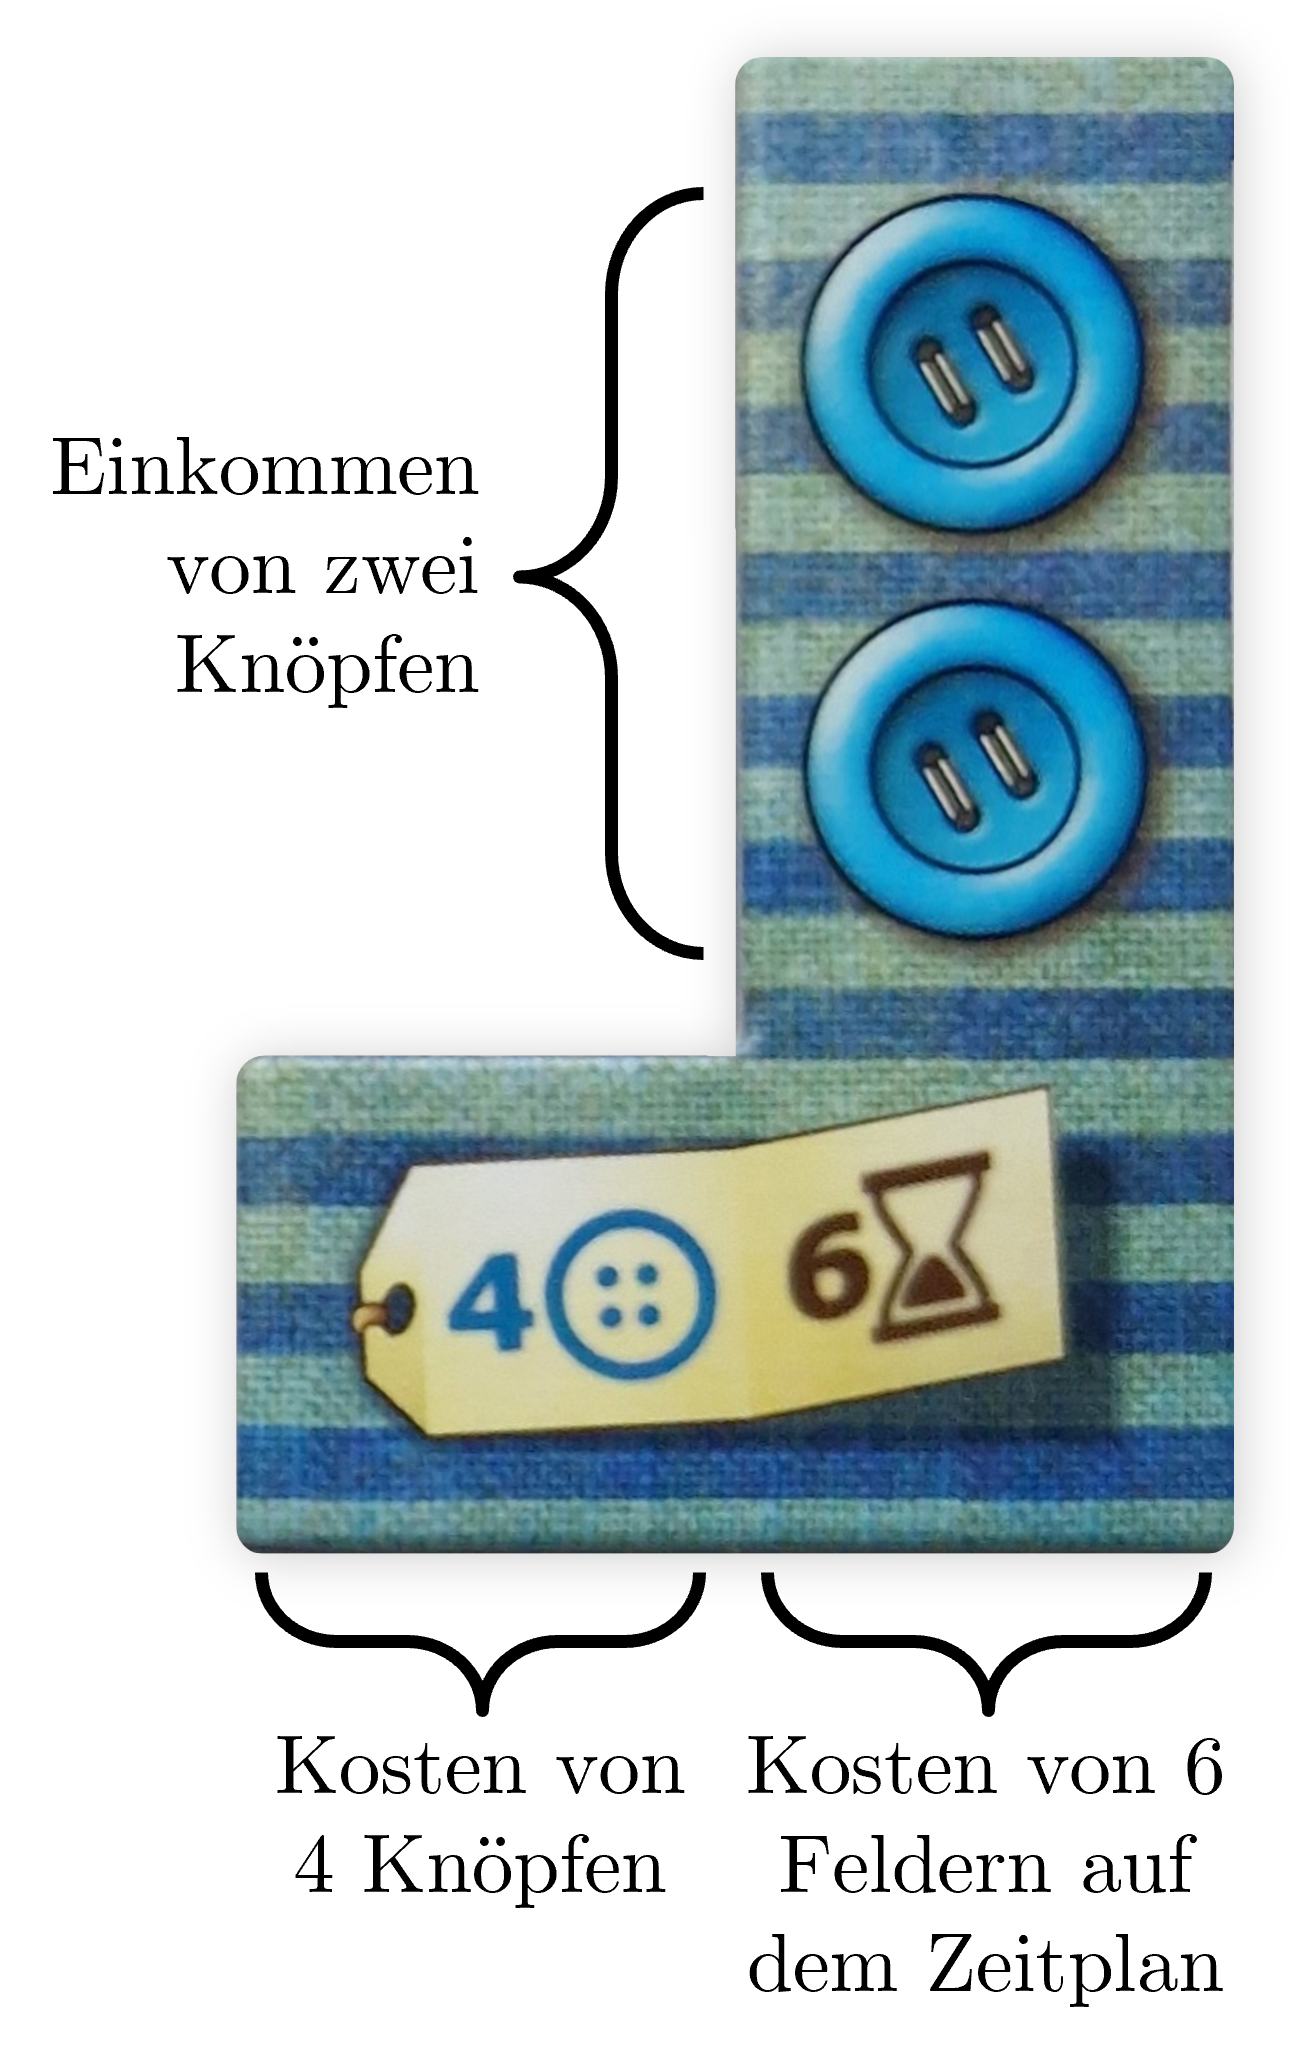
\includegraphics[width=0.3\textwidth]{res/pictures/annotated-patch.png}
    \caption{Flicken mit erklärender Beschriftung}
    \label{fig:patch-explanation}
\end{figure}

Während des Spielverlaufs rücken die Zeitstein der beiden Spieler immer weiter auf der Zeitleiste auf dem Zeitplan vor. Dort sind zwei Markierungen denen Beachtung geschenkt werden muss. Zum einen sind dort die Spezialflicken zu finden, welche der Spieler, der zuerst seinen Zeitstein über einen Spezialflicken zieht, für seinen Ablageplan verwenden und dort ablegen muss. Zum anderen sind Knöpfe auf der Zeitleiste zu erkennen. Wenn ein Zeitstein über ein solchen Knopf gezogen wird, bekommt derjenige Spieler ein Knopfeinkommen vom Vorrat in Höhe der Summe der Knöpfe, welche auf den Flicken auf seinem Ablageplan zu sehen sind. Ein Spieler, der nur den in Abbildung \ref{fig:patch-explanation} zu sehenden Flicken auf seinem Ablageplan liegen hat, würde somit ein Einkommen von 2 Knöpfen erhalten. \cite{2014.PatchworkSpielanleitung}

\pagebreak

\begin{wrapfigure}{r}{0.20\textwidth}
    \centering
    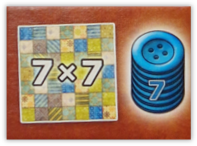
\includegraphics[width=0.18\textwidth]{res/pictures/assets/special-tile.png}
    % \vspace{-10pt}
    % Das folgende ist ein Trick, um "Abbilgung x.y" in eine
    % eigene Zeile zu packen. Der Text zwischen [ und ] steht
    % im Abbildungsverzeichnis. Der Text darunter wird
    % tatsächlich angezeigt.
    \caption[Sonderplättchen $7\times7$]{\unskip}
    Sonderplättchen $7\times7$
    \label{fig:special-tile}
\end{wrapfigure}

Bei dem Vorrat liegt das Sonderplättchen $7\times7$, in Abbildung \ref{fig:special-tile} zu sehen, welches der Spieler bekommt, der zuerst ein vollständig ausgefülltes $7\times7$-Quadrat aus Feldern auf seinem Ablageplan hat. Bei der Wertung am Ende des Spiels bringt dieses Sonderplättchen 7 Punkte. \cite{2014.PatchworkSpielanleitung}

Das Spiel endet, wenn die Zeitsteine der beiden Spieler das Zielfeld der Zeitleiste erreicht haben. Dabei verfallen überzählige Schritte und werden bei der Aktion \textbf{Vorrücken und Knöpfe erhalten} nicht ausgezahlt. \cite{2014.PatchworkSpielanleitung}

Zur Bestimmung des Gewinners müssen beide Spieler ihrer Knopfguthaben zählen, welches die Basis für ihren Punktestand darstellt. Falls das Sonderplättchen $7\times7$ ausgegeben wurde, wird dies auf den Punktestand des Spielers addiert. Vom Punktestand des Spielers werden nun für jedes freie Feld auf dem eigenen Ablageplan zwei Punkte abgezogen werden. Der Spieler mit der höchsten Gesamtpunktzahl ist Gewinner, bei Gleichstand gewinnt der Spieler, welcher zuerst das Zielfeld erreicht hat. \cite{2014.PatchworkSpielanleitung}

\subsection*{Ungenauigkeiten der Spielregeln}

In der Spielanleitung ist nicht genau beschrieben, was geschehen soll, wenn ein Spieler eine Spezialflicken legen muss, er jedoch auf seinem Ablageplan kein Feld mehr frei hat. Die Regel wird im Konsens so erweitert, dass falls dieser Fall eintrifft, der Spieler den Spezialflicken aus dem Spiel nimmt und neben sein Ablageplan legt. Auf die Wertung hat dies keinen Einfluss. \cite{2014.DiscussionSpecialPatch}

Außerdem wird in der Spielanleitung geschrieben, dass der Spieler, welcher \enquote{zuerst ein Quadrat von mindestens $7\times7$ Feldern auf seinem Ablageplan vollständig belegt hat} \cite{2014.PatchworkSpielanleitung}, das Sonderplättchen bekommt. Hier wird nicht ganz deutlich, wie genau diese Regel auszulegen ist. Die Regel wird im Konsens wie folgt interpretiert: Es muss kein vollständiges Quadrat ($8\times8$, $9\times9$) das $7\times7$-Quadrat umschließen, es reicht aus, wenn $7\times7$-Felder vollständig von Flicken bedeckt sind. Somit ist erlaubt, dass neben dem $7\times7$-Quadrat weitere Felder ausgefüllt sind und die gesamte Form auf dem Ablageplan kein Quadrat sein muss. \cite{2014.Discussion7x7}

\section{Spieltheoretische Analyse}

Patchwork ist ein \emph{sequentielles} 2\textendash{}Spieler\textendash{}Brettspiel. Sequentielle Spiele sind rundenbasierte Spiele, bei denen die Spieler nacheinander ziehen \cite[S. 53]{2014.GameTheoryThroughExamples}. Außerdem ist Patchwork ein Spiel mit \emph{perfekter Information}, \dash dass beide Spieler zu jeder Zeit genau wissen, was der andere Spieler getan hat und wie der jetzige Zustand des Spiels ist. Des Weiteren ist Patchwork ein \emph{Strategiespiel}. Wie für viele Strategiespiele typisch, enthält Patchwork auch keinen Zufall während des Spielablaufes. Die einzige Ausnahme ist vor dem Spielbeginn, da dort die Flicken in einer zufälligen Reihenfolge ausgelegt werden. Da beide Spieler in dem Brettspiel versuchen einen Sieg zu erreichen, handelt es sich weiterhin um ein \emph{Nullsummenspiel}. Bei Nullsummenspielen wird der Gewinn für einen Spieler als Verlust des anderen Spielers angesehen. Auch wenn das in Patchwork für einen einzelnen Spielzug nicht unbedingt der Fall sein muss, geht es bei Nullsummenspielen aber nur um das Gewinnen oder Verlieren des gesamten Spiels.

\subsection*{Anzahl der möglichen Startpositionen}

Das Brettspiel ist bis auf die Startposition der Spielteile deterministisch. Der einzige Zufallsfaktor beim Start ist das Auslegen der einzelnen Flicken im Kreis. Es gibt insgesamt 33 Flicken, welche ausgelegt werden müssen. Jedoch ist der kleinste Flicken, welcher nur 2 Felder auf einem Ablageplan einnimmt ($2\times1$ bzw. $1\times2$), immer an der gleichen Position direkt hinter der Spielfigur. Somit gibt es nur noch 32 Flicken, dessen Positionen angeordnet werden müssen. Eine solche Anordnug aller 32 Flicken auf 32 mögliche Positionen wird als \emph{Permutation} bezeichnet und besitzt $32! = 263.130.836.933.693.530.167.218.012.160.000.000 \approx 2,6 \cdot 10^{35}$ Möglichkeiten. Somit gibt es $2,6 \cdot 10^{35}$ mögliche Startpositionen.

\subsection*{Isomorphie der Zeitpläne}

Wie bereits in »\nameref{section:spielregeln}« erläutert, existieren zwei verschiedene Zeitpläne, welche jedoch nur anders gestaltet sind. Somit sind beide Zeitpläne isomorph zueinander, \dash sie weisen dieselbe Struktur auf, obwohl der konkrete Aufbau verschieden ist. Diese innere Struktur ist zusammen mit den beiden Zeitplänen in \ref{tabelle:isomorphie-zeitplan} veranschaulicht.

\begin{table}[!ht]
    \centering
    \begin{tabular}[t]{cc}
        \adjustbox{center, width=0.4735\textwidth, valign=m, margin=0 1ex 0 0}{\begin{tikzpicture}
                                                                                       \node [inner sep=0pt,,outer sep=0pt,clip,rounded corners=0.15cm] (image) at (0,0) {\includegraphics[width=0.625\textwidth]{res/pictures/assets/game-board-side-1.png}};
                                                                                       \drawshadow{image}
                                                                                   \end{tikzpicture}} &
        \adjustbox{center, width=0.4735\textwidth, valign=m, margin=0 1ex 0 0}{\begin{tikzpicture}
                                                                                       \node [inner sep=0pt,,outer sep=0pt,clip,rounded corners=0.15cm] (image) at (0,0) {\includegraphics[width=0.625\textwidth]{res/pictures/assets/game-board-side-2.png}};
                                                                                       \drawshadow{image}
                                                                                   \end{tikzpicture}} \\
        \multicolumn{2}{c}{\adjustbox{valign=m, margin=0 2ex 0 2ex}{Zugrundeliegende Struktur des Zeitplans:}}                                                                            \\
        \multicolumn{2}{c}{\adjustbox{width=0.97\textwidth}{
\includegraphics{res/pictures/time-board-structure.pdf}}}                                                                     \\
    \end{tabular}
    \vspace{5pt}
    \caption{Die Zeitpläne zusammen mit der zugrundeliegenden Struktur}
    \label{tabelle:isomorphie-zeitplan}
\end{table}

Aus diesem Grund kann Patchwork nachfolgend als ein Spiel betrachtet werden, da die Auswahl eines konkreten Zeitplans keinen Unterschied für die Betrachtung ausmacht.

\subsection*{Länge des Spiels}

In der Spieltheorie ist der Begriff eines Spielzuges nicht eindeutig. Ein Spielzug könnte eine einzelne Aktion eines Spielers sein, \zB das Auswählen und Legen eines Flickens in Patchwork von einem Spieler. Jedoch kann ein Spielzug auch so verstanden werden, dass beide Spieler eine Aktion machen müssen. So wird beispielsweise in rundenbasierten Spielen wie Schach ein Spielzug oft so angesehen, dass einmal die weiße und einmal die schwarze Seite gezogen haben müssen. Aufgrund dieser Zweideutigkeit wird ein Spielzug in der Spieltheorie mit einem \hyperref[text:ply]{\emph{Ply}} genauer definiert.

\begin{defStrich}[Ply]
    Ein Spielzug, welcher von einem Spieler gezogen wird, und stellt die kleinste mögliche Aktion in einem Spiel dar. \cite[S. 213]{1959.GameTheoryStudiesCheckers}
\end{defStrich}
\label{text:ply}
\vspace{-0.2cm}

Durch diese Definition kann genau definiert werden, was mögliche \hyperref[text:ply]{\emph{Plys}} in Patchwork sind. Die obige Definition für einen Spielzug, bei dem beide Spieler gezogen haben müssen, ist in Patchwork sowieso schwierig umzusetzen, da ein Spieler mehrere \hyperref[text:ply]{\emph{Plys}} hintereinander ausführen kann. Insgesamt gibt es drei mögliche Arten von \hyperref[text:ply]{\emph{Plys}} in Patchwork:

\begin{itemize}
    \item Vorrücken des Zeitsteins und Knöpfe erhalten
    \item Einen Flicken nehmen und auf dem Ablageplan platzieren
    \item Das Legen eines Spezialflicken auf den Ablageplan
\end{itemize}

Immer wenn ein Spieler an der Reihe ist, kann er zwischen dem Vorrücken und dem Platzieren von drei Flicken unterscheiden. Die Aktion einen Spezialflicken auf die Decke zu legen, kommt im Spiel immer genau fünfmal vor.

Patchwork endet, sobald beide Zeitsteine der Spieler das Zielfeld auf der Zeitleiste erreicht haben. Um ein möglichst langes Spiel zu spielen, muss also die Anzahl der Felder, die ein Spieler mit seinem Zeitstein pro \hyperref[text:ply]{\emph{Ply}} vorzieht, minimiert werden.

Für die Aktion \enquote{Einen Flicken nehmen und auf der Decke platzieren} ist die Anzahl der Felder immer durch den ausgewählten Flicken vorgegeben und beträgt mindestens 1 und maximal 6.

\pagebreak

Die Anzahl der Felder bei der Aktion \enquote{Vorrücken des Zeitsteins und Knöpfe erhalten} ist abhängig von der relativen Position der einzelnen Zeitsteine zueinander. Die maximale Anzahl an Feldern, die ein Zeitstein in einem Zug vorrücken kann, beträgt 7. Da immer ein Spielerwechsel stattfindet, sobald der Zeitstein des derzeitigen Spielers weiter vorrangeschritten ist als der Zeitstein des Gegners, muss für eine maximale Anzahl die Distanz zwischen den Zeitsteinen möglichst groß sein. Ein Zeitstein kann sich von dem anderem Zeitstein nur um maximal 6 Felder entfernen. Das ist der Fall, wenn der Flicken mit Zeitkosten 6 ausgewählt wird, während sich beide Zeitsteine auf demselben Feld befinden. Nach dieser Aktion ist der andere Spieler an der Reihe, welche sein Zeitstein um 7 Felder fortbewegen kann (Distanz von 6 Feldern $+$ 1 Feld, um weiter vorrangeschritten zu sein als der andere Zeitstein). Die minimale Anzahl an Felder bei der Vorrücken-Aktion beträgt 1 und kann bei drei Spielzuständen auftreten. Zuerst ist es möglich, dass beide Zeitsteine auf demselben Feld sind, sodass der Spieler, welcher an der Reihe ist, seinen Zeitstein nur 1 Feld vorrückt. Weiterhin ist es möglich, dass ein Zeitstein auf dem Feld vor dem Ziel ist, während der andere Spieler bereits im Ziel ist. In dieser Situation darf der Zeitstein auch nur um ein Feld vorgerückt werden. Zuletzt existiert noch die Situation am Spielanfang. Da hier auch beide Zeitsteine auf demselben Feld \textemdash{} dem Startfeld des Zeitplans \textemdash{} sind, darf der Startspieler den Zeitstein auch nur um ein Feld vorrücken.

Um die Länge des Spiels zu maximieren, sollte jeder Spieler so wenige Felder wie möglich vorrücken. Nutzt jeder Spieler immer die \enquote{Vorrücken des Zeitsteins und Knöpfe erhalten} Aktion, so gibt es insgesamt 54 \hyperref[text:ply]{\emph{Plys}}, da auf dem Zeitplan insgesamt 53 Felder sowie ein Start- und ein Zielfeld existieren. Während beim ersten und letzen \hyperref[text:ply]{\emph{Ply}} der Erste bzw. Zweite Spieler seinen Zeitstein nur um 1 Feld vorrückt, muss der Zeitstein während des Spiels immer 2 Felder vorgerückt werden, da die vorherige Aktion \textemdash{} auch eine \enquote{Vorrücken des Zeitsteins und Knöpfe erhalten} Aktion \textemdash{} impliziert, dass der Zeitstein des Gegners genau 1 Feld vor dem eigenen Zeitstein liegt.

\begin{table}[!ht]
    \centering
    \resizebox{\textwidth}{!}{
        \begin{tabular}[t]{c|c|c|c}
            \adjustbox{valign=t, raise=-16.25ex}{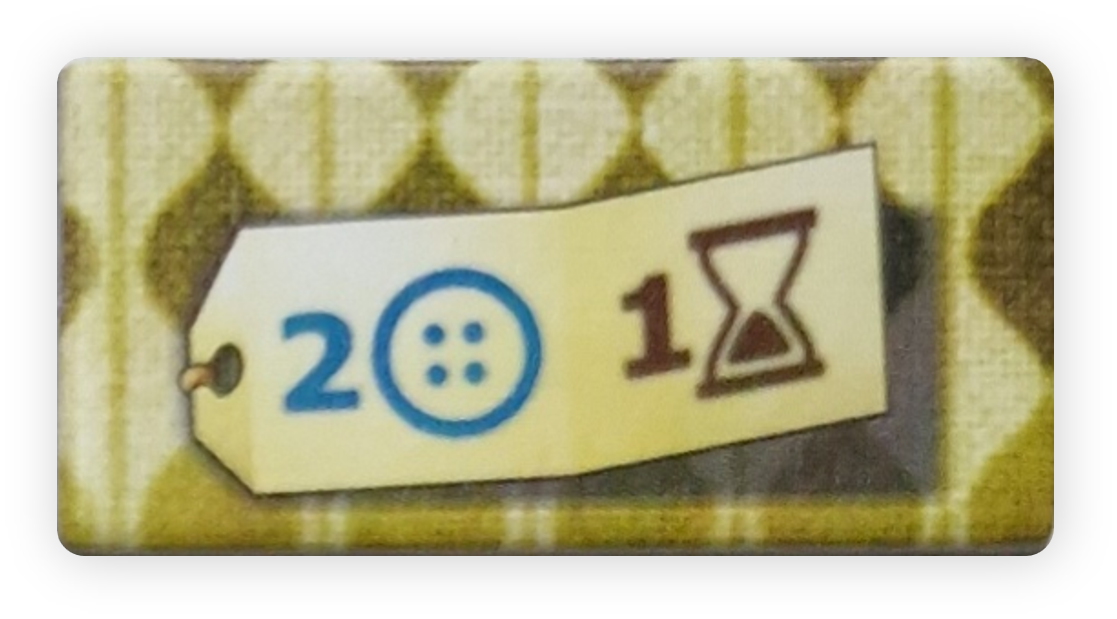
\includegraphics[width=0.2\textwidth]{res/pictures/assets/00-front.png}} &
            \adjustbox{valign=t, raise=0ex}{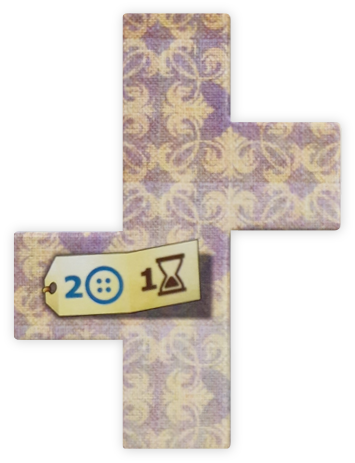
\includegraphics[width=0.3\textwidth]{res/pictures/assets/06-front.png}}      &
            \adjustbox{valign=t, raise=-9.05ex}{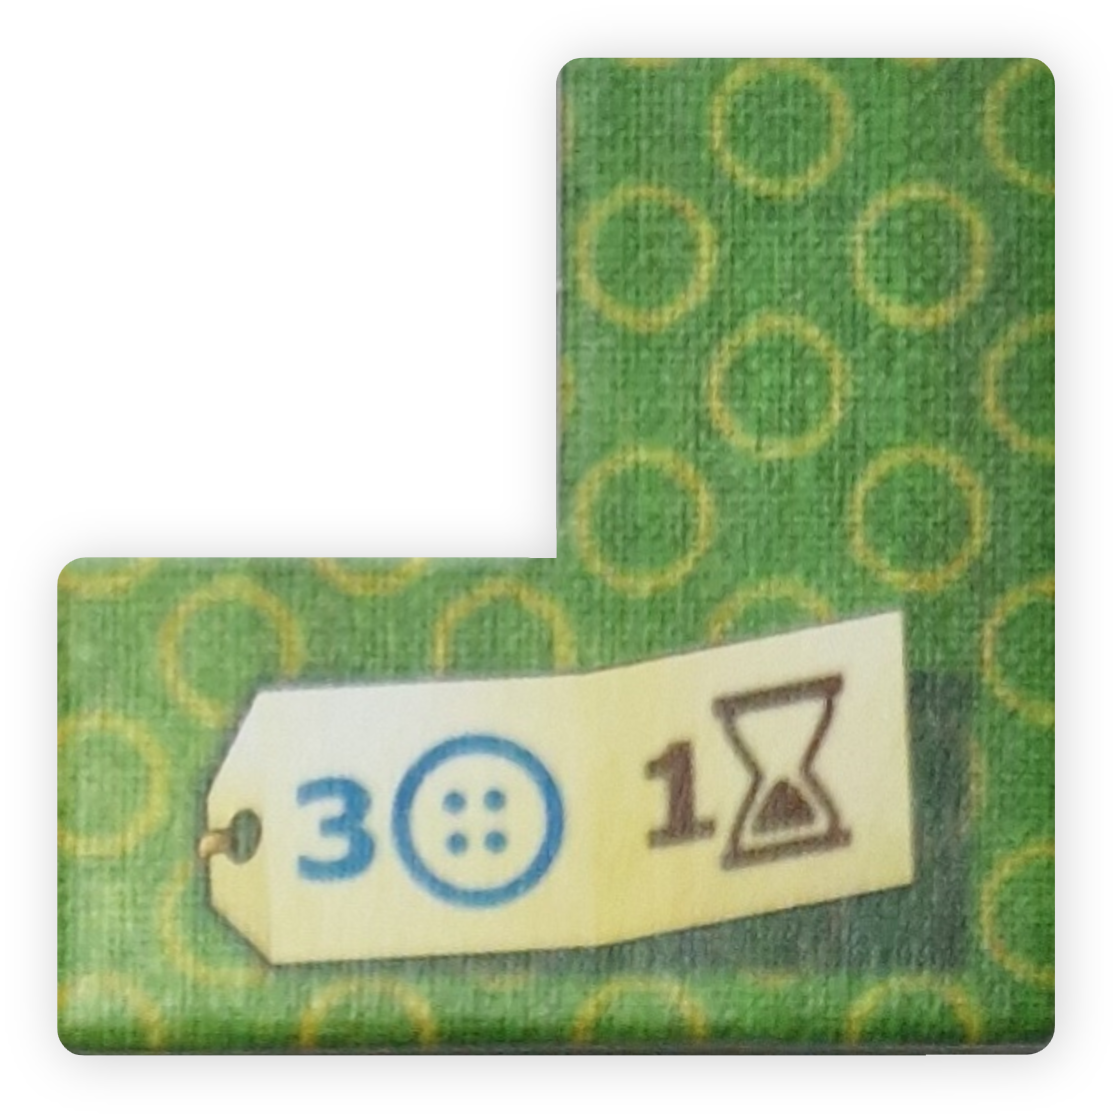
\includegraphics[width=0.2\textwidth]{res/pictures/assets/21-front.png}}  &
            \adjustbox{valign=t, raise=-16.25ex}{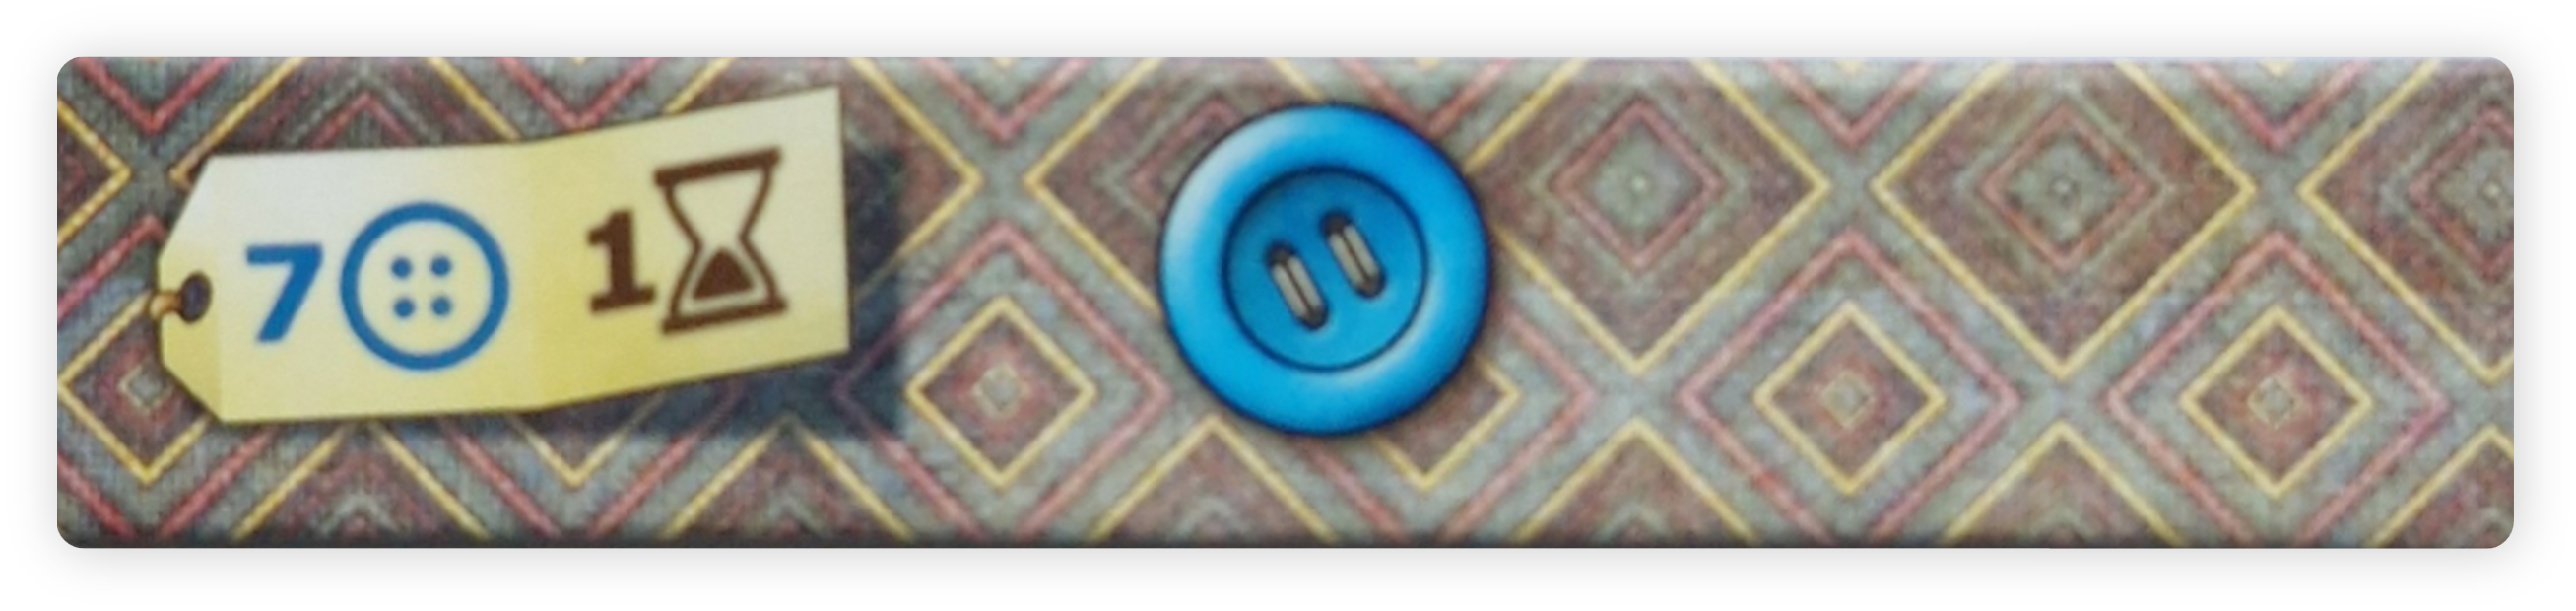
\includegraphics[width=0.5\textwidth]{res/pictures/assets/27-front.png}}   \\
        \end{tabular}
    }
    \vspace{5pt}
    \caption{Die vier Flicken mit Zeitkosten 1}
    \label{tabelle:flicken-mit-zeitkosten-1}
\end{table}

Die Zeitkosten bei der Aktion \enquote{Einen Flicken nehmen und auf der Decke platzieren} sind immer fest, wobei es insgesamt neun Flicken gibt, bei denen die Zeitkosten auch 2 betragen. So können optimal 9 Vorrücken-Aktionen durch die Auswahl dieser Flicken ersetzt werden. Weiterhin gibt es aber auch noch die vier in \ref{tabelle:flicken-mit-zeitkosten-1} dargestellten Flicken, welche nur Zeitkosten von 1 besitzen. Wird nun ein Vorrücken-\hyperref[text:ply]{\emph{Ply}} mit 2 Zeitkosten durch eine Kombination aus Flicken mit Zeitkosten 1 auswählen und auf der Decke Platzieren und anschließend ein Vorrücken-\hyperref[text:ply]{\emph{Ply}} mit Zeitkosten 1 ersetzt, ist das Spiel um 4 weitere \hyperref[text:ply]{\emph{Plys}} verlängert. Das ist möglich, da davon wie oben beschrieben der Zeitstein des derzeitigen Spielers immer direkt hinter dem Zeitstein des Gegners ist. Wird nun ein Flicken mit Zeitkosten 1 ausgewählt, befindet sich der Zeitstein des derzeitigen Spielers auf dem Zeitstein des Gegners. So kann ein Vorrücken-\hyperref[text:ply]{\emph{Ply}} mit Zeitkosten von 1 anstatt 2 ausgeführt werden. Da alle anderen Flicken höhere Zeitkosten verlangen, ist keine weitere Optimierung des Spiels hinsichtlich der der maximalen Länge mehr möglich.

Die maximale Länge des Brettspiels ergibt sich somit aus der Kombination der 54 Vorrücken-\hyperref[text:ply]{\emph{Plys}} zusammen mit den 4 zusätzlich gewonnenen \hyperref[text:ply]{\emph{Plys}} durch das Legen von Flicken mit Zeitkosten 1. Weiterhin kommen noch die fünf \hyperref[text:ply]{\emph{Plys}} für das Legen von Spezialflicken hinzu. Somit beträgt die maximale Länge von Patchwork \textbf{63} \hyperref[text:ply]{\emph{Plys}}.

\subsection*{Minimum und Maximum für die Anzahl an möglichen Aktionen \\ in einem \hyperref[text:ply]{Ply}}

Um die Komplexität von Patchwork zu untersuchen, ist es auch interessant zu betrachten, wie viele Auswahlmöglichkeiten einem Spieler bei seinem Zug zur Verfügung stehen.

Ist ein Spieler am Zug, kann er immer die Aktion \enquote{Vorrücken des Zeitsteins und Knöpfe erhalten} auswählen. Somit beträgt die minimale Anzahl an Aktionen mindestens 1. Dabei handelt es sich auch um das Minimum, da der derzeitige Spieler weniger Knöpfe im Vorrat haben kann, als die ersten 3 Flicken nach der Spielfigur an Knöpfen kostet. Somit kann der Spieler sich keinen der Flicken leisten und muss automatisch seinen Zeitstein vorrücken.

Eine obere Schranke für die maximal mögliche Anzahl an Aktionen ergibt sich als:

\vspace*{-0.45cm}
\begin{equation}
    \text{Obere Schranke}_{\text{Aktionen}} = \:
    \underset{\mathclap{\substack{\rotatebox[origin=c]{90}{\(\{ \)} \mathstrut \\ \text{Vorrücken}}}}{1}
    + \:
    \overset{\mathclap{\substack{\text{maximale Auswahlanzahl} \mathstrut \\ \text{Flicken} \mathstrut \\ \rotatebox[origin=c]{-90}{\(\{ \)}}}}{3} \:
    \times \:
    \max\limits_{\mathclap{\substack{\phantom{\text{\tiny m}} \\ f\, \in\, \text{Flicken}}}} \:\,
    \left\lvert\, \text{Platziermöglichkeiten}\left( f \right)\, \right\rvert
\end{equation}

Dabei ist eine $+1$ für die Aktion \enquote{Vorrücken des Zeitsteins und Knöpfe erhalten} vorhanden. Weiterhin gibt es für einen Spieler die Möglichkeit aus maximal 3 Flicken einen Flicken auszuwählen. Diese Anzahl wird multipliziert mit der maximalen Anzahl an Möglichkeiten, mit dem ein Flicken auf dem Ablageplatz platziert werden kann.

Um die maximale Anzahl an Platzierungsmöglichkeiten festzulegen, muss zuerst betrachtet werden, auf wie viele Arten ein Flicken auf die Ablagedecke gelegt werden kann. Die Operationen, welche vor dem Platzieren auf einen Flicken angewendet werden können, sind Drehungen und Spiegelungen, wodurch die Flicken identisch zur Diedergruppe $D_4$ sind. Die Gruppe besteht aus 8 Elementen \cite[S. 33]{2015.AbstractAlgebra}, was somit gleichzeigt die maximale Anzahl an Transformationen für ein Flicken ist. Jedoch muss beachtet werden, dass die Flicken die maximale Anzahl nicht erreichen müssen. Zum Beispiel existiert ein $2\times2$ Flicken, welcher im Sinne der Diedergruppe 8 Ausprägungen besitzt, jedoch auf der Ablagedecke mit allen Drehungen und Spiegelungen immer genau dieselben Felder bedeckt. Für die maximale Platzierungsanzahl ist aber nur relevant, dass ein Flicken existiert, welcher bei allen 8 Transformationen eine andere Anordnung aufweist. Dieser Flicken existiert und ist in Abbildung \ref{fig:diedergruppe} dargestellt.

\begin{figure}[!ht]
    \centering
    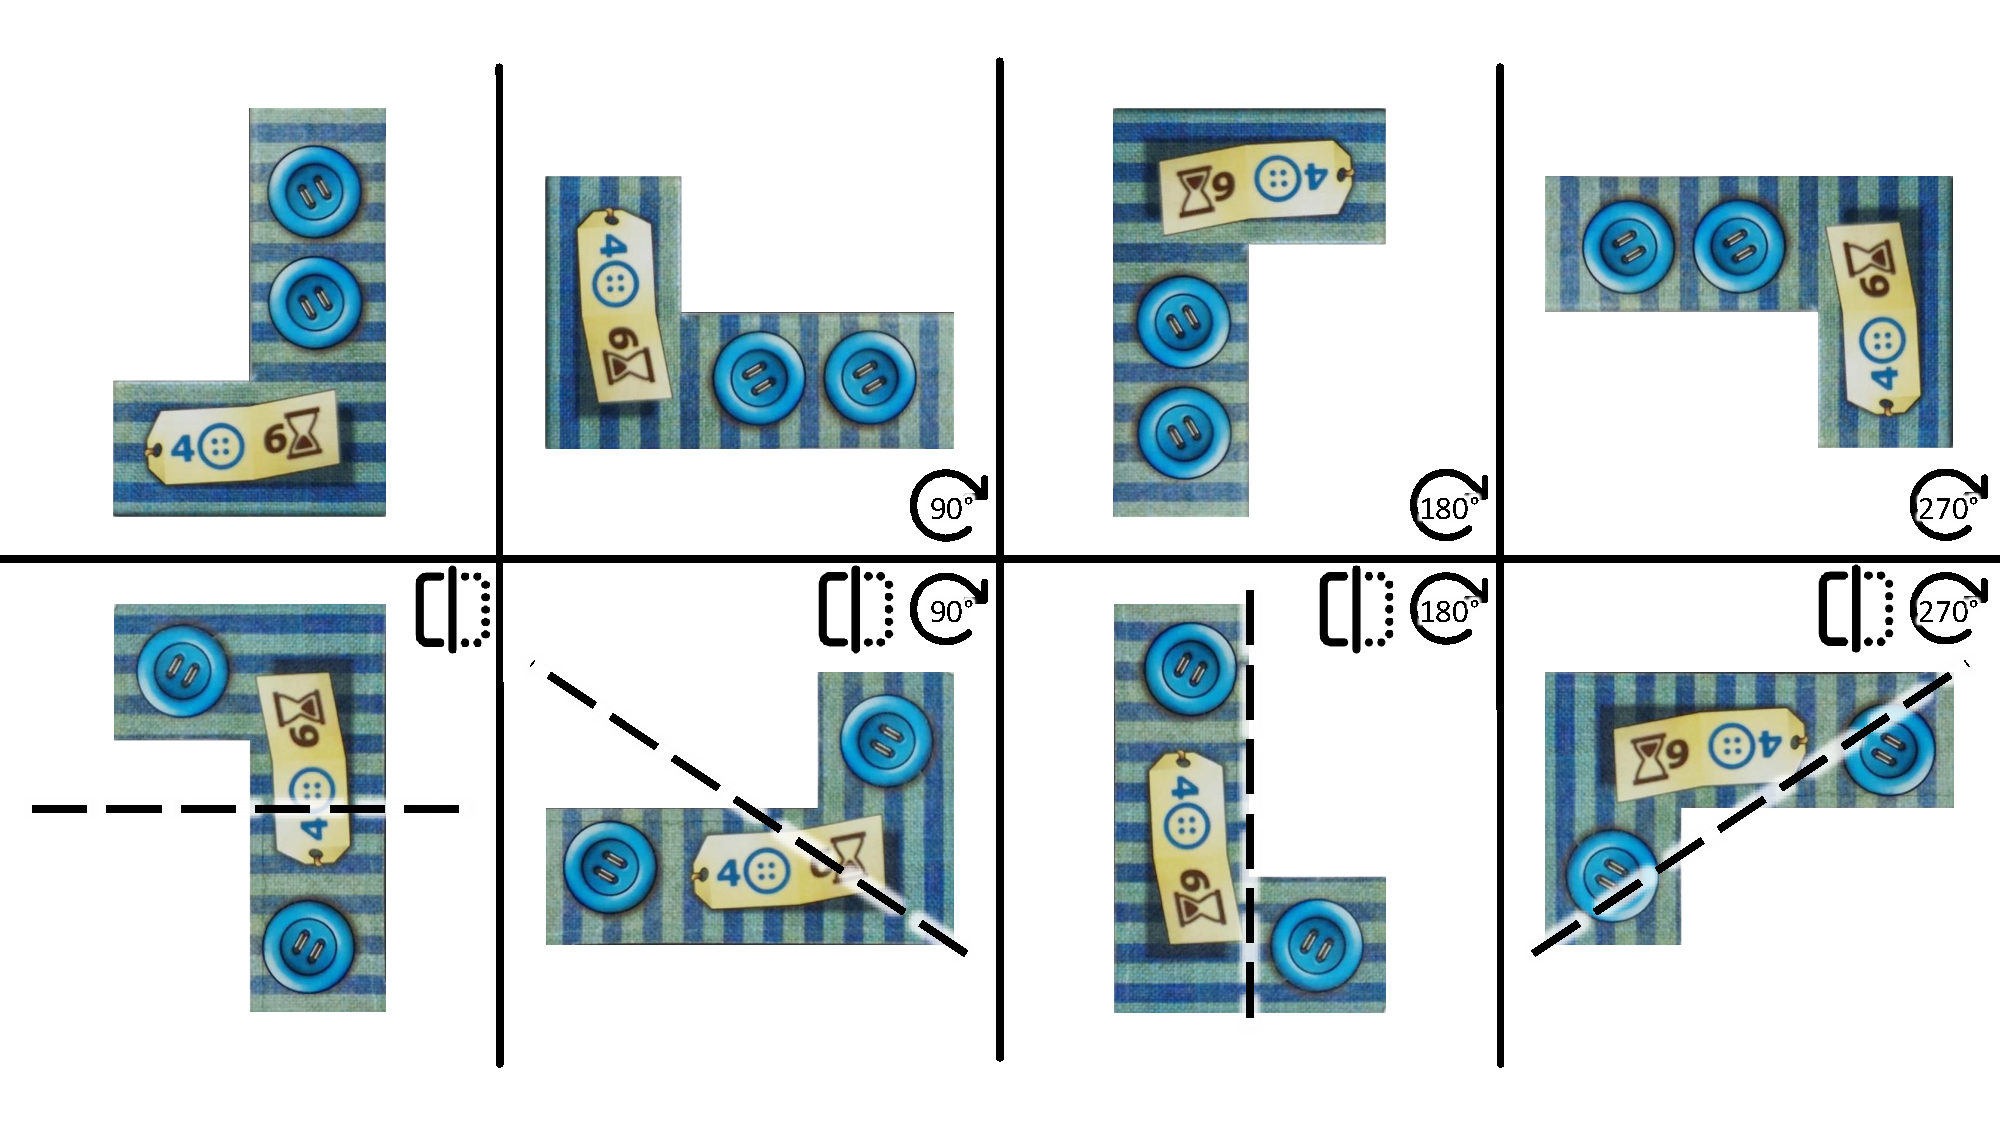
\includegraphics[width=0.995\textwidth]{res/pictures/dihedral-group.pdf}
    \vspace*{-0.5cm}
    \caption{Flicken mit 8 verschiedenen Transformationen}
    \label{fig:diedergruppe}
\end{figure}

Weiterhin gibt es verschiedene Möglichkeiten den transformierten Flicken auf den $9\times9$ Felder großen Ablageplan zu legen. Die Möglichkeiten lassen sich dabei einfach wie in Term \ref{eqn:ablagefeld-platzierungen} in Abhängigkeit von der Breite und Höhe des Flickens sowie der Anzahl der unterschiedlichen Transformationen berechnen.

\vspace*{-0.45cm}
\begin{equation}
    \label{eqn:ablagefeld-platzierungen}
    \left( 9 - \text{Höhe}  + 1 \right) \cdot
    \left( 9 - \text{Breite} + 1 \right) \cdot
    \left\lvert\, \text{Transformationen} \,\right\rvert
\end{equation}

Die Anzahl der Platzierungsmöglichkeiten für den in \ref{fig:diedergruppe} dargestellten $3\times 2$ großen Flicken beträgt somit $\left( 9 - 3 + 1 \right) \cdot \left( 9 - 2 + 1 \right) \cdot 8 = 448$. Jedoch muss für die Platzierungsmöglichkeiten beachtet werden, dass sich die Anzahl reduziert, je größer ein Flicken ist. Somit muss für alle Flicken, dessen Höhe $\le 3$ und Breite $\le 2$ ist \textemdash{} wobei mindestens eine der beiden Ungleichungen strikt (also $<$) sein muss \textemdash{} überprüft werden, ob mehr Platzierungsmöglichkeiten bestehen als bei dem Flicken von \ref{fig:diedergruppe}. Es existieren nur 3 Flicken dieser Art, welche in Tabelle \ref{tabelle:kleine-flicken} dargestellt sind. Jeder dieser Flicken weißt dabei durch die geringere Anzahl an verschiedenen Transformationsmöglichkeiten insgesamt weniger Platzierungsmöglichkeiten auf als der Flicken in \ref{fig:diedergruppe}.

\begin{table}[!ht]
    \centering
    \begin{tabular}[t]{c|c}
        Flicken                                                                                                                        & Platzierungsmöglichkeiten \\ \hline
        \hspace*{0.5cm} \adjustbox{valign=m}{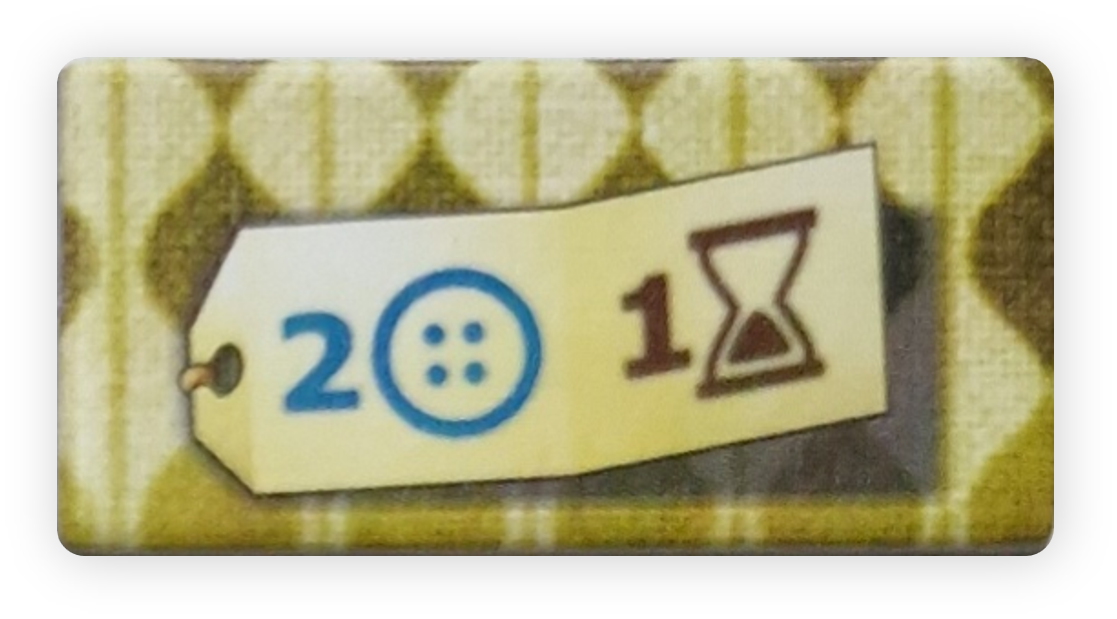
\includegraphics[width=0.15\textwidth]{res/pictures/assets/00-front.png}} \hspace*{0.5cm} & \hspace*{0.5cm}
        $\left( 9 - 1 + 1 \right) \cdot \left( 9 - 2 + 1 \right) \cdot 2 = 144$ \hspace*{0.5cm}                                                                    \\ \hline
        \hspace*{0.5cm} \adjustbox{valign=m}{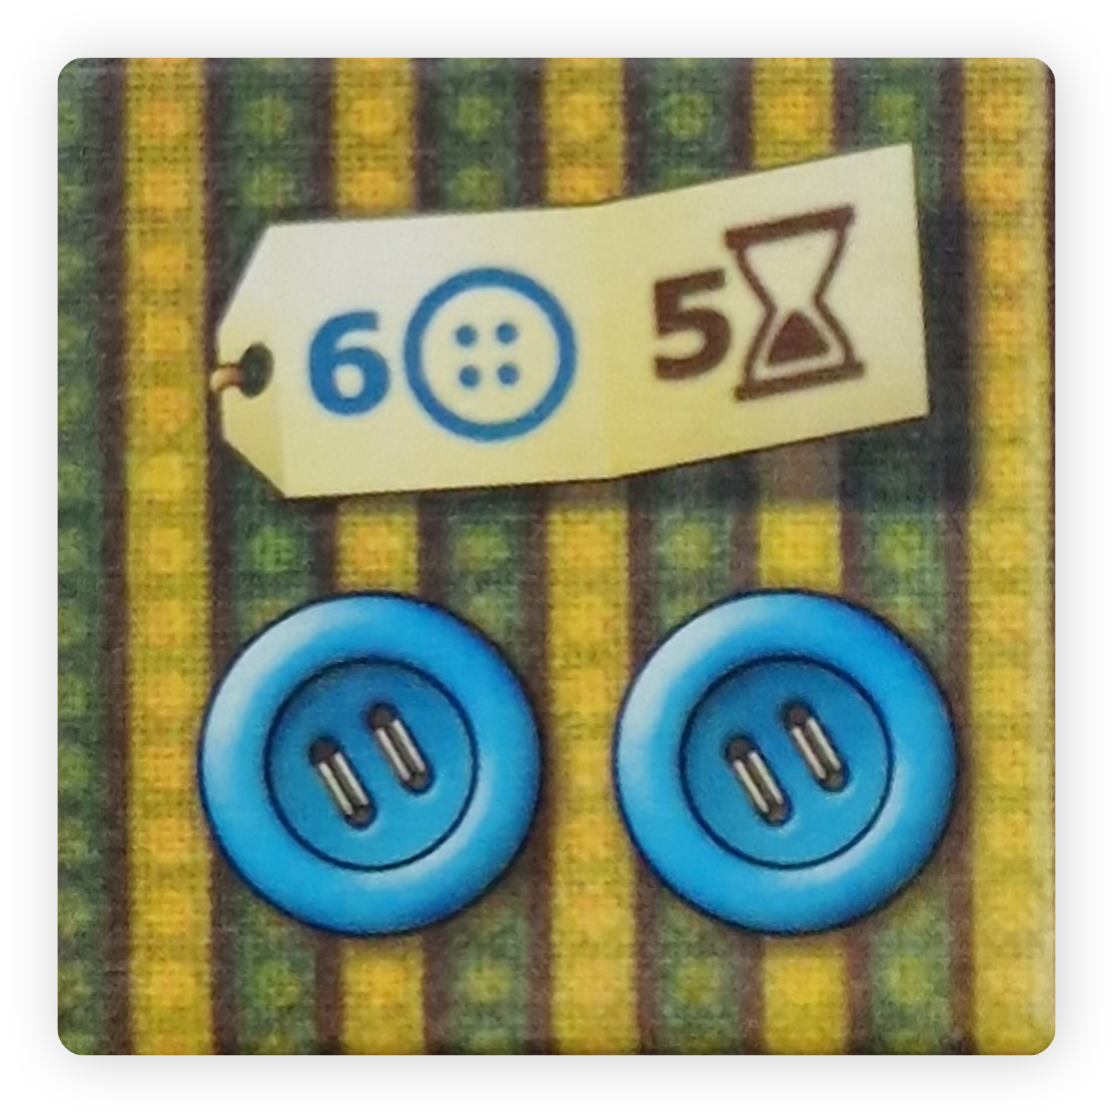
\includegraphics[width=0.15\textwidth]{res/pictures/assets/09-front.png}} \hspace*{0.5cm} & \hspace*{0.5cm}
        $\left( 9 - 2 + 1 \right) \cdot \left( 9 - 2 + 1 \right) \cdot 1 = 64$ \hspace*{0.5cm}                                                                     \\ \hline
        \hspace*{0.5cm} \adjustbox{valign=m}{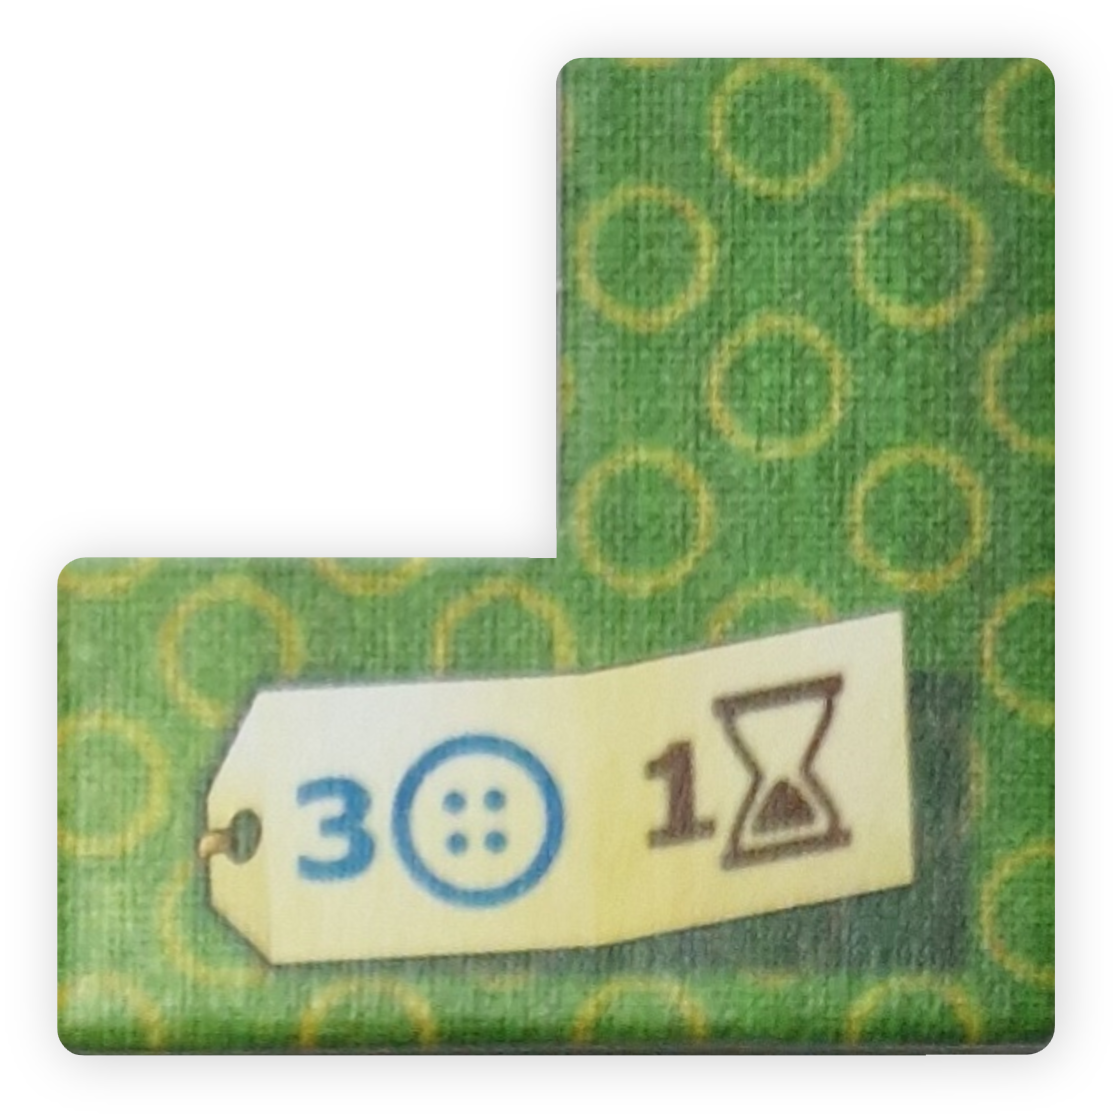
\includegraphics[width=0.15\textwidth]{res/pictures/assets/21-front.png}} \hspace*{0.5cm} & \hspace*{0.5cm}
        $\left( 9 - 2 + 1 \right) \cdot \left( 9 - 2 + 1 \right) \cdot 4 = 256$ \hspace*{0.5cm}                                                                    \\
    \end{tabular}
    \vspace{5pt}
    \caption{Platzierungsmöglichkeiten der kleineren Flicken}
    \label{tabelle:kleine-flicken}
\end{table}

\begin{wrapfigure}{r}{0.25\textwidth}
    \centering
    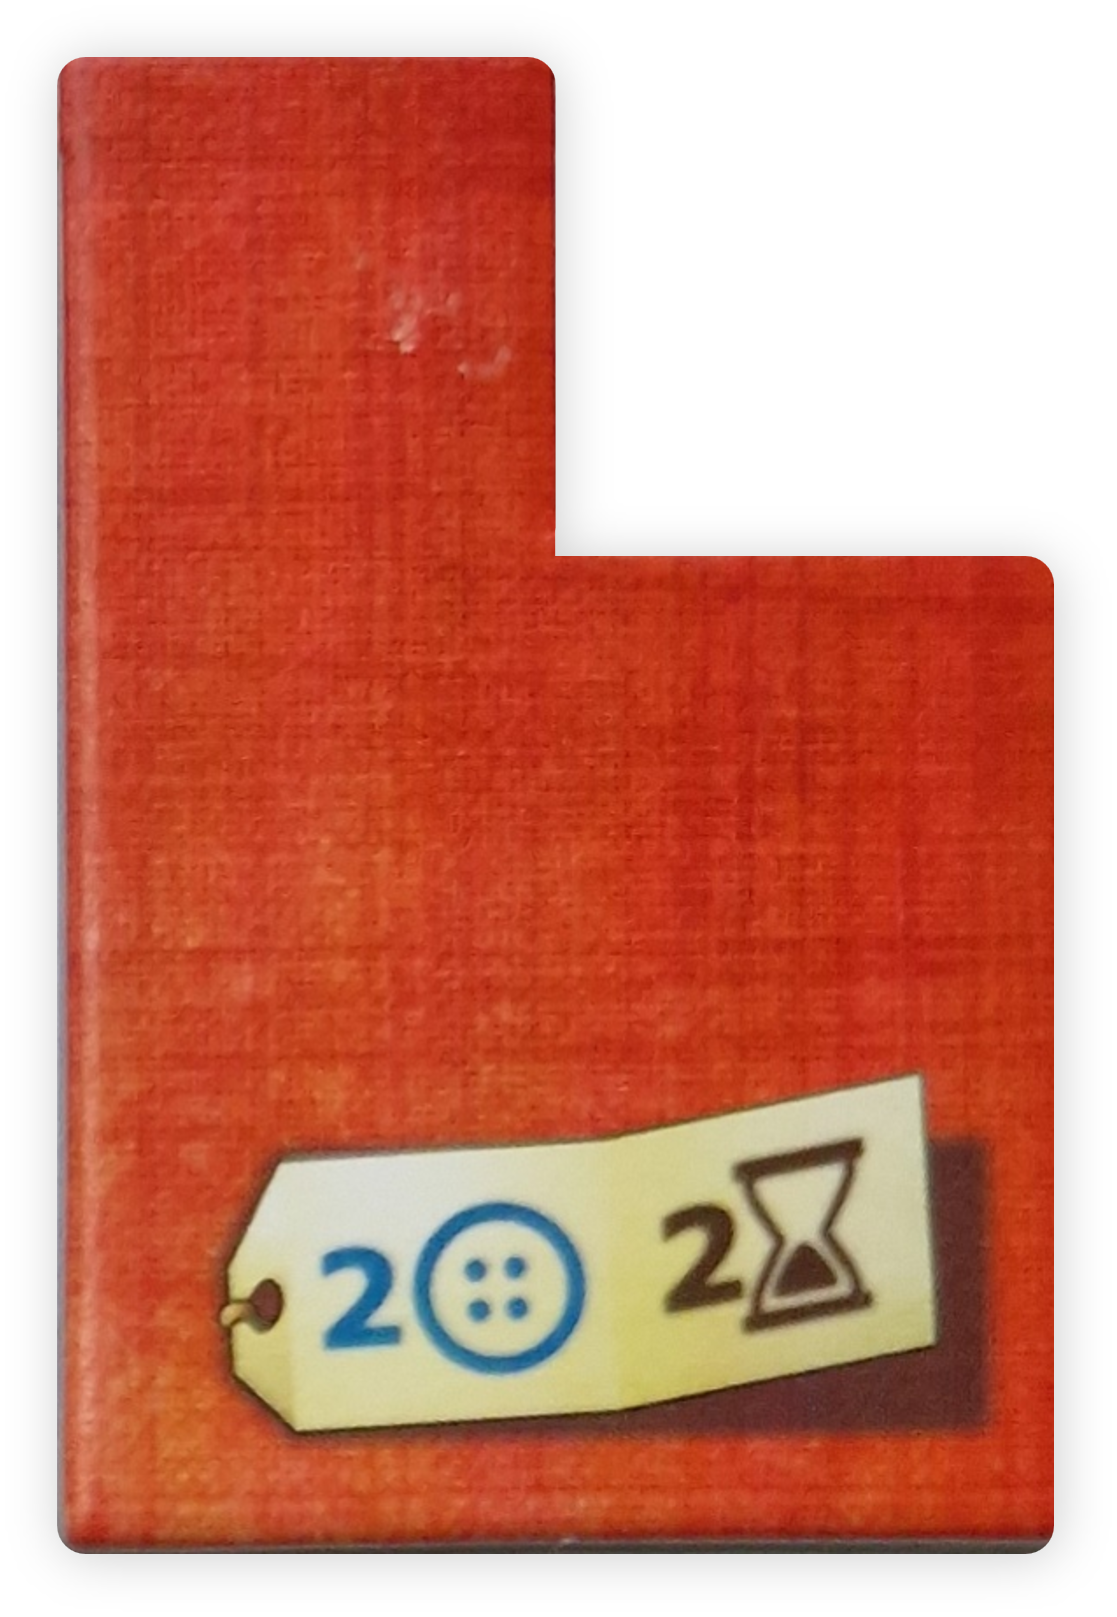
\includegraphics[width=0.12\textwidth]{res/pictures/assets/08-front.png}

    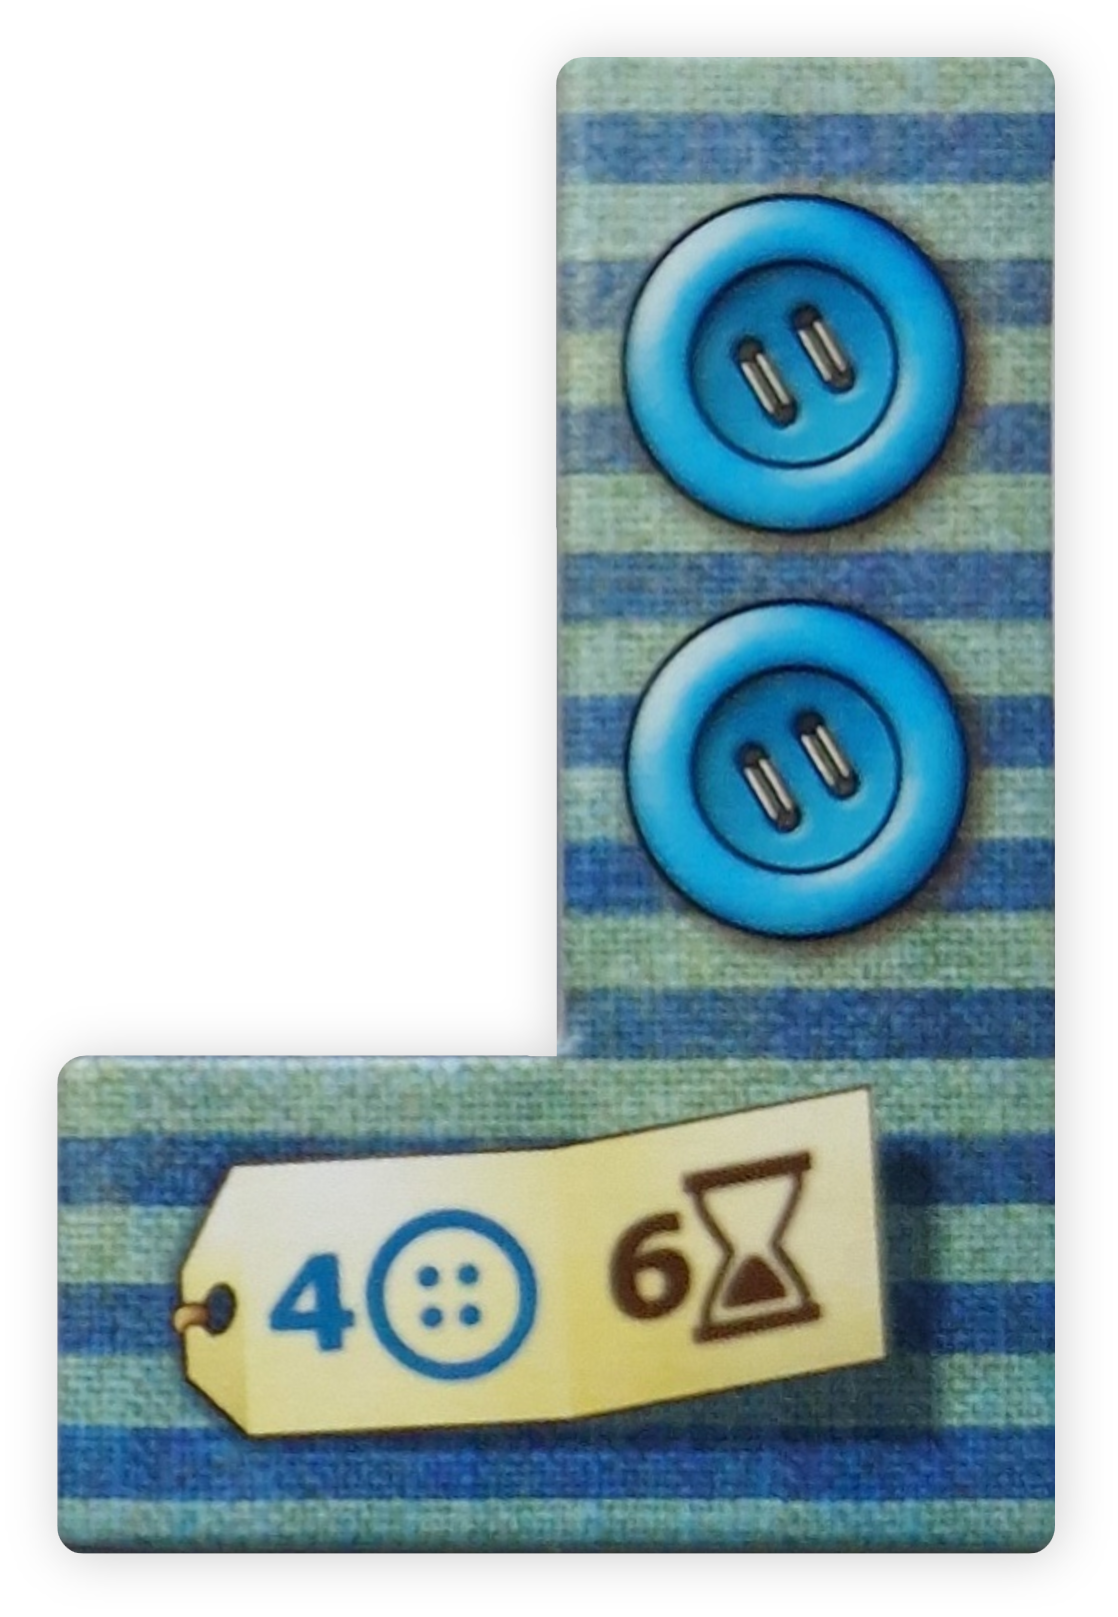
\includegraphics[width=0.12\textwidth]{res/pictures/assets/14-front.png}

    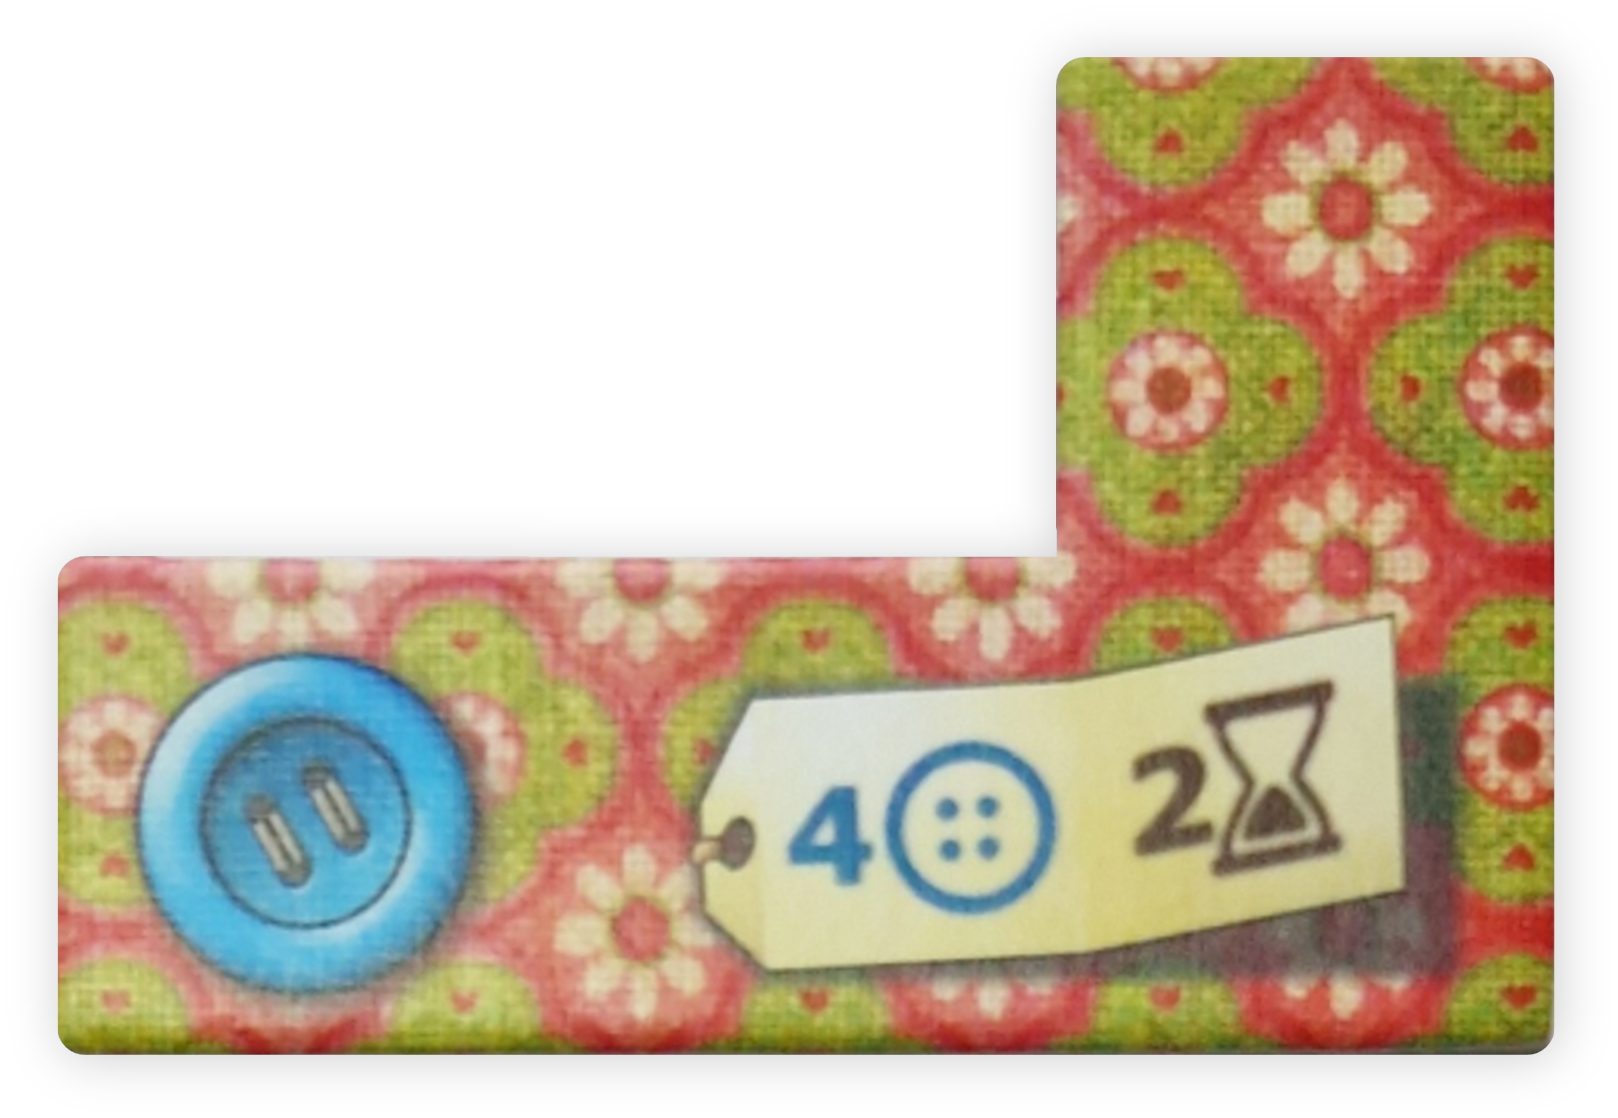
\includegraphics[width=0.18\textwidth]{res/pictures/assets/19-front.png}
    % \vspace{-10pt}
    % Das folgende ist ein Trick, um "Abbilgung x.y" in eine
    % eigene Zeile zu packen. Der Text zwischen [ und ] steht
    % im Abbildungsverzeichnis. Der Text darunter wird
    % tatsächlich angezeigt.
    \caption[Alle Flicken mit 448 Platzierungsmöglichkeiten]{\unskip}
    Alle Flicken mit 448 Platzierungsmöglichkeiten
    \label{fig:flicken-mit-448}
\end{wrapfigure}

Um sicherzustellen, dass die maximale Platzierungsmöglichkeit auf dem Ablageplan auch tatsächlich für die drei zur Verfügung stehenden Flicken auftreten kann, müssen mindestens drei unterschiedliche Flicken mit einer Größe von $3 \times 2$ bzw. $2 \times 3$ existieren, welche 448 Möglichkeiten zur Platzierung auf dem Ablageplan besitzen. Das ist der Fall, wie die Flicken in Abbildung \ref{fig:flicken-mit-448} zeigen.

Um die maximale Anzahl an möglichen Aktionen festzustellen muss zuletzt noch das Platzieren von Spezialflicken als Sonderfall betrachtet werden. Da alle Spezialflicken eine Größe von $1 \times 1$ besitzen, unterscheiden sich die Transformationen nicht hinsichtlich der Platzierung auf dem Ablageplan. Somit gibt es $9 \cdot 9 \cdot 1 = 81$ mögliche Aktionen einen Spezialflicken auf dem Ablageplan zu platzieren.

Das tatsächliche Maximum für die mögliche Anzahl an Aktionen ergibt sich dann als das Maximum der normalen Aktionen und der Aktion \enquote{Legen eines Spezialflicken} wie in \ref{eqn:max-aktionen} dargestellt ist:

\begin{equation}
    \label{eqn:max-aktionen}
    \text{Maximum}_{\text{Aktionen}} = \max \left\{ 1 + 3 \cdot 448\, ,\, 81 \right\} = 1345
\end{equation}

Dabei ist anzumerken, dass die maximale Anzahl an Platzierungsmöglichkeiten für normale sowie Spezialflicken nur genau dann möglich ist, wenn der Ablageplan noch leer ist. Weiterhin kann die maximale Auswahlmöglichkeit auch bereits direkt am Anfang des Spiels geschehen, da alle Flicken in \ref{fig:flicken-mit-448} mit dem Startbudget von 5 Knöpfen gekauft werden können.

\subsection*{Obere und untere Schranke für die Wertung eines Spielers}

In dieser Sektion wird eine obere und eine untere Schranke für die Wertung eines Spielers am Ende des Spiels festgesetzt. Da sich die Wertung aus dem am Ende vorhandenen Vorrat an Knopf-Plättchen und der Anzahl der Lücken im eigenen Spielbrett zusammensetzt, werden zunächst die maximal möglichen Werte für diese beiden Komponenten bestimmt. Anschließend werden die Schranken für die Wertung eines Spielers am Ende des Spiels festgesetzt.

\subsection*{Maximal mögliche Anzahl zusätzlichen Knopf-Plättchen an bei der Knopf-Wertung}

TODO:

Max Button Income
% /// The maximum amount of button income a player can have is bounded
% /// by the number of tiles in the quilt board.
% ///
% /// The highest possible upper bound that is realistic would therefore be `81`
% /// (The amount of tiles in the quilt board). But this would require that
% /// all patches that are layed out have at least the same button income as
% /// the amount of tiles they cover. This is not true for any patch in the
% /// game.
% ///
% /// Therefore variable uses a more conservative upper bound of `32`.
% /// For this the patches were ordered by the percentage of button income in
% /// relation to the amount of tiles they cover. Then the first patches were
% /// chosen until the amount of tiles covered was `>= 81`. With this a
% /// maximum button income of 33 as upper bound was found.
% ///
% /// Here is the list of all patches and the patches that were chosen ordered
% /// by the percentage of button income in relation to the amount of tiles:
% ///
% /// ```txt
% /// index:  4, tiles: 4, buttons: 3, percentage: 0.75
% /// index:  1, tiles: 5, buttons: 3, percentage: 0.6
% /// index:  3, tiles: 6, buttons: 3, percentage: 0.5
% /// index:  9, tiles: 4, buttons: 2, percentage: 0.5
% /// index: 12, tiles: 6, buttons: 3, percentage: 0.5
% /// index: 14, tiles: 4, buttons: 2, percentage: 0.5
% /// index: 17, tiles: 5, buttons: 2, percentage: 0.4
% /// index: 18, tiles: 5, buttons: 2, percentage: 0.4
% /// index: 29, tiles: 5, buttons: 2, percentage: 0.4
% /// index: 13, tiles: 6, buttons: 2, percentage: 0.3333333333333333
% /// index: 15, tiles: 6, buttons: 2, percentage: 0.3333333333333333
% /// index: 30, tiles: 6, buttons: 2, percentage: 0.3333333333333333
% /// index: 19, tiles: 4, buttons: 1, percentage: 0.25
% /// index: 26, tiles: 4, buttons: 1, percentage: 0.25
% /// index: 28, tiles: 4, buttons: 1, percentage: 0.25
% /// index: 10, tiles: 5, buttons: 1, percentage: 0.2
% /// index: 27, tiles: 5, buttons: 1, percentage: 0.2
% /// --------------- CUTOFF AFTER 84 >= 81 TILES COVERED ---------------
% /// index: 31, tiles: 5, buttons: 1, percentage: 0.2
% /// index: 16, tiles: 6, buttons: 1, percentage: 0.16666666666666666
% /// index: 32, tiles: 6, buttons: 1, percentage: 0.16666666666666666
% /// index: 20, tiles: 7, buttons: 1, percentage: 0.14285714285714285
% /// index:  2, tiles: 8, buttons: 1, percentage: 0.125
% /// index:  0, tiles: 2, buttons: 0, percentage: 0
% /// index:  5, tiles: 6, buttons: 0, percentage: 0
% /// index:  6, tiles: 6, buttons: 0, percentage: 0
% /// index:  7, tiles: 7, buttons: 0, percentage: 0
% /// index:  8, tiles: 5, buttons: 0, percentage: 0
% /// index: 11, tiles: 6, buttons: 0, percentage: 0
% /// index: 21, tiles: 3, buttons: 0, percentage: 0
% /// index: 22, tiles: 5, buttons: 0, percentage: 0
% /// index: 23, tiles: 3, buttons: 0, percentage: 0
% /// index: 24, tiles: 4, buttons: 0, percentage: 0
% /// index: 25, tiles: 3, buttons: 0, percentage: 0
% /// ```
% ///
% /// But this is not the least upper bound (supremum) as the tiles covered
% /// are `84` in the end and not `81`. The actual supremum is a button
% /// income of `32`. This is the case because the most one can cover below
% /// the limit of 81 tiles is reached is only a button income of `32`.
% /// Then at least 79 tiles are covered and all patches with 2 tiles or less
% /// do not have any button income. To show that this is actually not only
% /// the supremum but a reachable maximum a quilt board has to be constructed
% /// that has a button income of 32. This is done in the following:
% ///
% /// ```txt
% /// 28 28 28 28 10 10 10 XX 13
% /// 19 19 19 10 10 13 13 13 13
% /// 19 04 18 18 18 18 12 12 13
% /// 04 04 18 XX 12 12 12 12 14
% /// 04 30 29 29 29 17 14 14 14
% /// 30 30 30 29 17 17 17 03 03
% /// 30 26 30 29 01 17 03 03 03
% /// 26 26 15 15 01 01 03 09 09
% /// 26 15 15 15 15 01 01 09 09
% ///
% /// where the tiles covered with XX are still free and all the other tiles
% /// have the id of the patch that covers them.
% /// ```
% ///
% /// This quilt board has a button income of 32, has a time cost of 66 and
% /// covers at least 79 tiles but can be filled up with two special patches
% /// to cover the full quilt board. While this is a maximum that can be
% /// created on the quilt board, it is not achievable in the game as the
% /// time cost of 66 is greater than the allowed time cost of 54.
% ///
% /// TODO: improve the bound even more
% ///

\subsection*{Maximal mögliche Anzahl an Knopf-Plättchen}


Bounds for lowest possible score, highest possible score, max button income, max button balance

Max button balance
TODO: take update from zobrist hash in rust implementation
% /// The maximum button balance a player can have is bounded by the game.
% ///
% /// * A player has `5` buttons at the start of the game.
% /// * There are only `9` button income triggers that can yield a maximum amount
% ///   of `33` buttons each (see `MAX_BUTTON_INCOME` estimate below).
% /// * The player can get `1` button income for every tile he walks on the
% ///   time track with the walking action. There are `54` tiles on the time track.
% /// * The only other income source are the `7` buttons from a full quilt board.
% ///
% /// Because of this the maximum button balance a player can have is bounded
% /// by `5 + 9 · 33 + 7 + 54 · 1 = 363`. This is a upper bound and not the
% /// actual maximum because of the same reason as the `MAX_BUTTON_INCOME`
% /// estimate below. Furthermore the player can only choose between the
% /// walking action and the action to place a tile. Therefore he cannot get
% /// both at the same time. It would probably be possible to lower the bound
% /// to `5 + 9 · 33 + 7 + 54 · 1 = 309` (remove the walking actions) and
% /// still be correct. But to be safe the bound is kept at `363`.


MAX possible score
363 = same as max button balance

min score
0 als bound für income + -81*2 als Punkte am Ende

-81*2 + 0 = -162

nicht realistisch, da man immer durch laufen mindestens 1 punkte bekommt. einzige möglichkeit punkte loszuwerden ist das quilt board zu füllen